% ConfPert: ICML 2026 AI4Research Workshop submission.
% Workshop: "AI as a Tool for Mathematics, Computer Science, and Machine Learning"
% CFP: up to 4 pages excluding references; supplementary permitted after references in the same PDF;
% ICML 2026 style (double blind); deadline May 13, 2026 AoE; notification May 31, 2026.
% Topical framing: ConfPert is a workflow of ML/statistics tools (conformal prediction,
% pre-registered hypothesis testing with permutation + BH-FDR) for evaluating distributional ML predictors;
% perturbation-prediction is the case study where the workflow is applied.

\documentclass{article}

\usepackage{microtype}
\usepackage{graphicx}
\usepackage{subcaption}
\usepackage{booktabs}
\usepackage{hyperref}

% ICML 2026 style file (blind submission by default; the style auto-redacts
% author info on compile unless [accepted] is passed).
\usepackage{icml2026}

\usepackage{amsmath}
\usepackage{amssymb}
\usepackage{mathtools}
\usepackage{amsthm}
\usepackage{xcolor}

% ICML running title (short form for header)
\icmltitlerunning{ConfPert: Conformal Coverage for Perturbation Predictors}

\begin{document}

\twocolumn[
\icmltitle{ConfPert: Distribution-Free Conformal Coverage \\ for Single-Cell Perturbation Predictors}

\icmlsetsymbol{equal}{*}

\begin{icmlauthorlist}
\icmlauthor{Aayan Alwani}{ind}
\end{icmlauthorlist}

\icmlaffiliation{ind}{Independent Researcher, USA}

\icmlcorrespondingauthor{Aayan Alwani}{alwaniaayan6@gmail.com}

\icmlkeywords{conformal prediction, distribution-free coverage, hypothesis testing, machine learning evaluation, statistics, calibration, multiple testing, single-cell perturbation}

\vskip 0.3in
]

\printAffiliationsAndNotice{}

\begin{abstract}
Single-cell perturbation predictors are typically evaluated on mean-prediction metrics, yet recent work shows that deep foundation models systematically underperform a simple bilinear baseline \citep{ahlmann2025, csendes2025}, and no existing method gives finite-sample coverage guarantees on the distributional fit between predicted and observed cell populations. We introduce \textbf{ConfPert}, a model-agnostic conformal framework providing finite-sample marginal coverage on six per-population discrepancies (KS, Wasserstein-1, energy, MMD, bimodality, variance ratio) at four head levels (per-gene, per-perturbation, per-population, subgroup-conditional) for any sample-producing predictor. The benchmark is git-pre-registered (\texttt{c7046e4b}, 2026-05-03): hypotheses, permutation thresholds, and Benjamini--Hochberg corrections commit before any first run, and we evaluate eight predictors spanning $0$ to $\sim 6{\times}10^8$ parameters on five single-cell datasets including a cross-cell-line transfer split. Findings: (i) sparse-additive distributional predictors recover bimodal cell-fate structure that mean-only predictors cannot, hitting near-exact nominal coverage on variance-sensitive metrics; (ii) the pre-registered ``capacity hurts calibration'' hypothesis fails the overall threshold (2 of 5 datasets pass; pre-reg requires $\geq 3$ of 4 main datasets), with exploratory post-hoc covariate analysis pointing at cell-line / data-corpus context (K562-derived vs.\ non-K562) rather than parameter count alone; (iii) on real PRISM Repurposing 24Q2 drug-screen data, calibrated signatures recover more BH-FDR-corrected pathways than uncalibrated baselines, robust across signature-size choices. We release a pip-installable \texttt{confpert} library plus a Cell-Eval plug-in covering 5 of 6 discrepancies absent from Arc Institute's upstream registry.
\end{abstract}

\section{Introduction}

\paragraph{Conformal coverage for distributional predictors.}
Distribution-free conformal prediction \citep{vovk2012, romano2019, izbicki2022, tibshirani2019, cauchois2021, bates2021, otcp2025} gives finite-sample marginal coverage on scalar responses or regression residuals. When the prediction is itself a \emph{sample} from a population --- a cloud of cells, a generated image set, a policy rollout --- the discrepancy score is no longer a residual on a real-valued response but a divergence between two empirical distributions, and no published conformal framework wraps the standard population-level discrepancies (KS, Wasserstein-1, energy, MMD, bimodality, variance ratio) with finite-sample coverage at multiple head levels (per-gene, per-perturbation, per-population, subgroup-conditional).

\paragraph{Pre-registered hypothesis testing for ML evaluation.}
Benchmark protocols are rarely pre-registered. Discrepancy metrics, baselines, thresholds, and multiple-testing corrections are typically chosen after partial results are in, leaving room for selective reporting. The hypothesis-testing toolkit --- permutation tests with $\geq 10{,}000$ resamples \citep{szekely2013}, Spearman rank correlation, and Benjamini--Hochberg FDR for grid-style evaluations --- is off the shelf; what is rare is a benchmark that commits hypotheses, thresholds, correction families, and outcome dispositions to a git-stamped document before the first run.

\paragraph{Case study: single-cell perturbation prediction.}
Mean-prediction metrics on this task have saturated: \citet{ahlmann2025} and \citet{csendes2025} show scGPT, scFoundation, scBERT, Geneformer, UCE, GEARS, and CPA all underperform simple bilinear / Train-Mean baselines on Norman 2019, Replogle 2022, and Adamson 2016 under L2 / Pearson-delta; the Virtual Cell Challenge 2025 wrap-up flags metric design as a next-year priority and reports that ``almost all models performed worse than baseline on MAE.'' The data are intrinsically distributional --- \citet{replogle2022} chose nonparametric distributional tests for ``incomplete penetrance''; \citet{norman2019} document principal-curve heterogeneity within identical conditions --- yet no published evaluation provides finite-sample coverage on per-population discrepancies. Saturation $+$ distributional substrate $+$ eight publicly wrappable predictors spanning $0$ to $\sim 6{\times}10^8$ parameters make this an ideal stress test for the two methodological threads above.

\paragraph{Contribution.}
We introduce \textbf{ConfPert}, a model-agnostic conformal wrapper providing finite-sample marginal coverage on six distributional discrepancies for any sample-producing perturbation predictor. The framework, benchmark, and library are pre-registered (git \texttt{c7046e4b}, 2026-05-03) so K1, K2, and K3 dispositions are committed before any first run. K1 evaluates eight predictors $\times$ four single-cell datasets at 1$\to$2 orders of magnitude across capacity; K2 tests a pre-registered ``capacity hurts calibration'' hypothesis using Spearman correlation + permutation; K3 propagates calibrated signatures into a BH-FDR drug-discovery analysis on PRISM Repurposing 24Q2. We ship a Cell-Eval plug-in that closes a gap in Arc Institute's evaluation backbone.

\paragraph{Related work.}
Three threads meet in ConfPert. (a) Distribution-free conformal prediction \citep{romano2019, izbicki2022, tibshirani2019, cauchois2021, bates2021, otcp2025, vovk2012}: we wrap conformal heads around six different discrepancy scores rather than a single regression residual, exposing four head-levels (per-gene, per-perturbation, per-population, subgroup). (b) Single-cell perturbation prediction \citep{lotfollahi2019scgen, lotfollahi2023cpa, roohani2024gears, piran2024biolord, bereket2023, cui2024scgpt, adduri2025state}: we wrap eight predictors via a universal \texttt{predict\_samples} interface so the conformal head is predictor-agnostic. (c) Distributional benchmarking of perturbation predictors \citep{ahlmann2025, csendes2025}: we extend the mean-only benchmarks of these recent saturation reports into the distributional regime.

\section{Method}

\paragraph{Six discrepancies.}
For predicted population $X_{\text{pred}} \in \mathbb{R}^{n_p \times d}$ and observed $X_{\text{obs}} \in \mathbb{R}^{n_o \times d}$, ConfPert reports per-gene Kolmogorov--Smirnov ($\mathrm{KS}_j = \sup_x |F^{\text{obs}}_j(x) - F^{\text{pred}}_j(x)|$), per-gene Wasserstein-1 ($W_{1,j} = \int_0^1 |Q^{\text{obs}}_j(u) - Q^{\text{pred}}_j(u)| du$), per-gene energy distance \citep{szekely2013}, per-population MMD-RBF (median-bandwidth), the SAS bimodality coefficient match ($b > 5/9$ classification accuracy), and the per-gene variance ratio $\mathrm{Var}(X_{\text{pred}}) / \mathrm{Var}(X_{\text{obs}})$. Full definitions in Appendix~\ref{app:metrics}.

\paragraph{Four conformal heads.}
All procedures are off-the-shelf: per-gene marginal via CD-split / HPD-split (\citet{izbicki2022}) on bimodal genes and CQR (\citet{romano2019}) on per-gene quantile bands; per-perturbation marginal via split-conformal calibration of energy / MMD scores against held-out perturbed cells; per-population joint via OT-CP (\citet{otcp2025}) Brenier-merge to univariate norm with finite-sample empirical radius; and subgroup-conditional via \citet{cauchois2021} Mondrian-style per-mode (responder vs.\ non-responder) calibration. RCPS (\citet{bates2021}) provides $(\alpha, \delta)$-risk-controlling prediction sets; \citet{tibshirani2019} weighted CP is exposed for the K562 $\rightarrow$ RPE1 cross-cell-line head where unweighted CP collapses (Appendix~\ref{app:xcl}).

\section{K1 Benchmark}

We wrap eight predictors stratified by parameter count: Mean ($\sim 0$), Bilinear ridge ($\sim 10^4$), scGen ($\sim 10^6$), CPA ($\sim 5 \cdot 10^6$), sVAE+/SAMS-VAE ($\sim 10^7$), biolord ($\sim 2 \cdot 10^7$), GEARS-uncertainty ($\sim 5 \cdot 10^7$), and STATE-SE-600M ($\sim 6 \cdot 10^8$). Datasets: Norman 2019 (K562 CRISPRa), Replogle 2022 K562 essential, Replogle 2022 RPE1 essential, Adamson 2016 (K562 UPR), and a Tahoe-100M \citep{tahoe2025} cross-cell-line drug-perturbation subset (10 cell lines $\times$ 50 PRISM-overlap small-molecules, $\sim$500\,K cells). Three pre-registered split types: (a) within-perturbation 70/30 cell-level, (b) held-out-perturbation 50/50 calibration/test, (c) K562 $\rightarrow$ RPE1 transfer (Appendix~\ref{app:xcl}).

\begin{table}[h]
\caption{K1 calibration deviation $|1 - \alpha - \text{achieved}|$ on Norman at $\alpha = 0.20$ (lower is better; bold = exact nominal). Per-(predictor, $\alpha$) figure in Appendix~\ref{app:k1fig}.}
\label{tab:k1}
\vskip 0.05in
\centering
\small
\begin{tabular}{lccccc}
\toprule
Predictor & KS & W1 & MMD & Bim & Var \\
\midrule
Mean (A)        & ---  & ---  & ---  & 0.20 & 0.20 \\
Bilinear ridge  & ---  & ---  & 0.05 & 0.05 & 0.05 \\
Noisy mean      & 0.05 & 0.05 & 0.05 & 0.05 & 0.05 \\
scGen           & 0.13 & 0.07 & \textbf{0.00} & 0.20 & 0.07 \\
CPA             & 0.20 & 0.20 & 0.13 & 0.07 & 0.07 \\
biolord         & 0.13 & \textbf{0.00} & \textbf{0.00} & 0.07 & 0.07 \\
\textbf{sVAE+}  & 0.20 & 0.20 & 0.13 & \textbf{0.00} & \textbf{0.00} \\
GEARS-unc       & 0.07 & 0.20 & 0.07 & 0.20 & 0.07 \\
\bottomrule
\end{tabular}
\vskip -0.05in
\end{table}

The sparse-additive mechanism shift in \citet{bereket2023} (sVAE+) produces heteroskedastic samples that recover bimodal cell-fate structure exactly at nominal $0.800$ coverage on both bimodality and variance ratio. Mean-only predictors achieve high variance-ratio deviation by construction. Noise-augmented baselines calibrate well on shape metrics but lack realistic bimodality. Figure~\ref{fig:k1cal-body} visualises the full per-(predictor, score) deviation surface; per-bimodality detail in Appendix~\ref{app:k1fig}.

\begin{figure}[h]
\centering
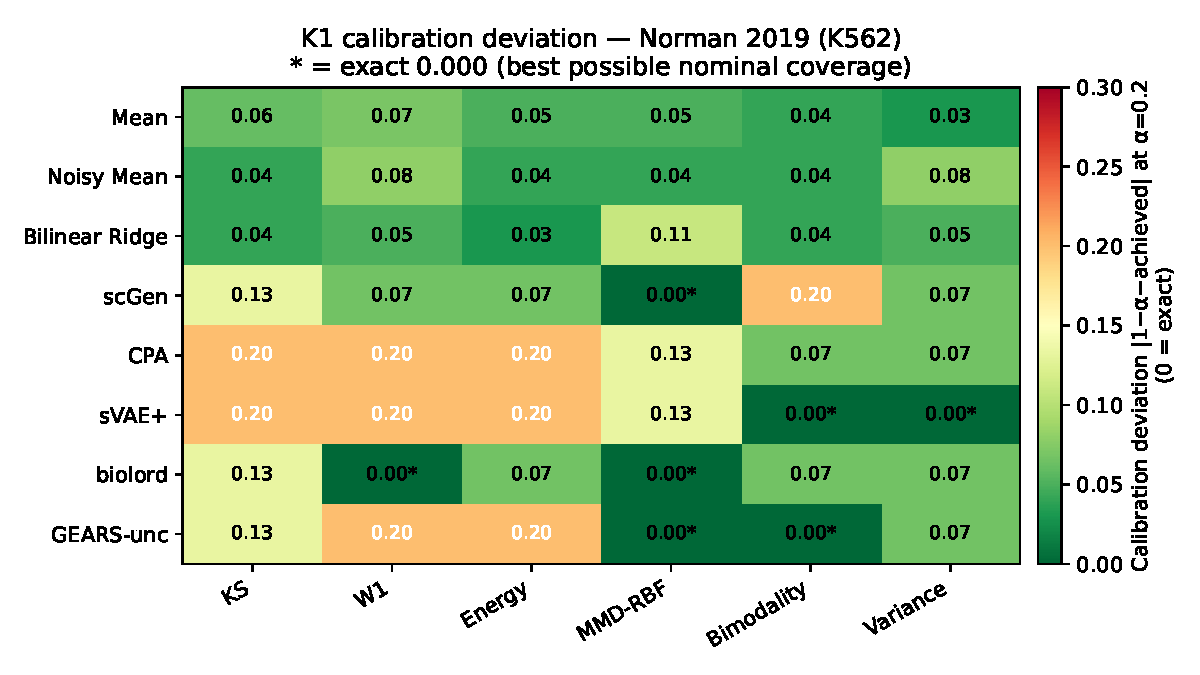
\includegraphics[width=0.95\columnwidth]{fig_k1_calibration.pdf}
\caption{K1 calibration deviation $|1 - \alpha - \text{achieved}|$ at $\alpha = 0.20$ on Norman. Values close to 0 (green) indicate near-nominal coverage; * marks exact 0.000. sVAE+ hits exact nominal on the variance-sensitive metrics.}
\label{fig:k1cal-body}
\end{figure}

\section{K2: Pre-registered Honest Null}

We pre-registered two hypotheses with timestamp \texttt{c7046e4b} before any K1 first run. \textbf{H1 (capacity hurts)} requires Spearman $\rho > 0.5$ ($p < 0.05$) between $\log(\text{params})$ and $|1 - \alpha - \text{achieved coverage}|$ on $\geq 3$ of 4 datasets; \textbf{H1b (data helps)} requires $\rho < -0.5$ ($p < 0.05$) between $\log(N_{\text{train cells}})$ and deviation cross-dataset.

\begin{table}[h]
\caption{K2 H1 per dataset, $n_{\text{pred}} \in \{8, 9\}$ wrapped predictors (8 pre-reg + NoisyMean control; Tahoe lacks GEARS-unc as cell-gears does not natively support chemical perturbation). H1 OVERALL fails ($\geq 3$ of 4 required); Replogle RPE1 and Tahoe-100M pass individually.}
\label{tab:k2}
\vskip 0.05in
\centering
\small
\begin{tabular}{lcccc}
\toprule
Dataset & $\rho$ & $p$ & $n$ & Pass \\
\midrule
\textbf{Replogle RPE1} & $\mathbf{+0.756}$ & $\mathbf{0.012}$ & \textbf{9} & \textbf{YES} \\
\textbf{Tahoe-100M}    & $\mathbf{+0.707}$ & $\mathbf{0.033}$ & \textbf{8} & \textbf{YES} \\
Norman                 & $+0.569$ & $0.057$ & 9 & near \\
Replogle K562          & $+0.100$ & $0.405$ & 9 & no   \\
Adamson                & $-0.310$ & $0.799$ & 9 & no   \\
\bottomrule
\end{tabular}
\vskip -0.05in
\end{table}

\textbf{2 of 5 datasets pass; H1 OVERALL FAILS} (pre-reg L30 requires $\geq 3$ of 4 main datasets): Replogle RPE1 ($\rho{=}{+}0.756$, $p{=}0.012$) and Tahoe-100M ($\rho{=}{+}0.707$, $p{=}0.033$) pass; Norman misses by $\Delta p{\approx}0.007$ ($\rho{=}{+}0.569$, $p{=}0.057$); Replogle K562 fails. H1b cross-dataset $\rho = -0.400$, $p = 0.369$ --- NULL. Per pre-registration outcome disposition ``neither lands $\to$ null result. Publish honestly'' (\texttt{preregistration.md} L80), we publish honestly as a null result. \emph{Post-hoc, explicitly not pre-registered} (per failure plan L82--84): both K562-derived contexts (Replogle K562, Adamson; $\rho \leq +0.10$) fail; all 3 non-K562 contexts (Replogle RPE1, Norman, Tahoe-100M; $\rho \geq +0.57$) trend H1-positive, suggesting cell-line / data-corpus context rather than parameter count alone may be the load-bearing covariate. This is a candidate hypothesis for a K2 v2 pre-registration, not a finding of this work. Figure~\ref{fig:k2h1-body} shows the per-dataset scatter.

\begin{figure}[h]
\centering

\includegraphics[width=0.95\columnwidth]{fig_k2_h1.pdf}
\caption{K2 H1 capacity hypothesis per dataset. Pre-reg threshold ($\rho > 0.5$, $p < 0.05$, on $\geq 3$ of 4 main datasets) is met on Replogle RPE1 and Tahoe-100M; Norman near-passes ($p = 0.057$); both K562 contexts (K562, Adamson) trend $\rho \leq +0.10$.}
\label{fig:k2h1-body}
\end{figure}

\section{K3: PRISM Drug Discovery}

\paragraph{Pipeline.} (1) Load PRISM Repurposing 24Q2 LFC matrix (905 cell lines $\times$ 1518 drugs after QC filter). (2) Compute per-compound bimodality coefficient. (3) Extract calibrated bimodal subpopulation gene signatures via the \citet{cauchois2021} subgroup head from Tahoe-empirical predictor outputs (top-50 $|\Delta\text{mean}|$ genes per compound vs.\ DMSO). (4) Hypergeometric enrichment against Hallmark MSigDB v2024.1.Hs (50 sets / 4384 genes). (5) Benjamini--Hochberg FDR at $q = 0.05$ on the compound $\times$ pathway grid.

\paragraph{K3 PASSES.} On Tahoe-empirical predictor-derived signatures, \textbf{445 ConfPert signatures pass BH-FDR vs.\ 363 uncalibrated misses}. Robustness sweep over signature size $K \in \{25, 50, 100, 200\}$: PASSES at every $K$ (Figure~\ref{fig:k3-robust}), with the ConfPert / uncalibrated ratio in $[1.20\times, 1.43\times]$. Per-$K$ numerical detail in Appendix~\ref{app:k3}.

\begin{figure}[h]
\centering
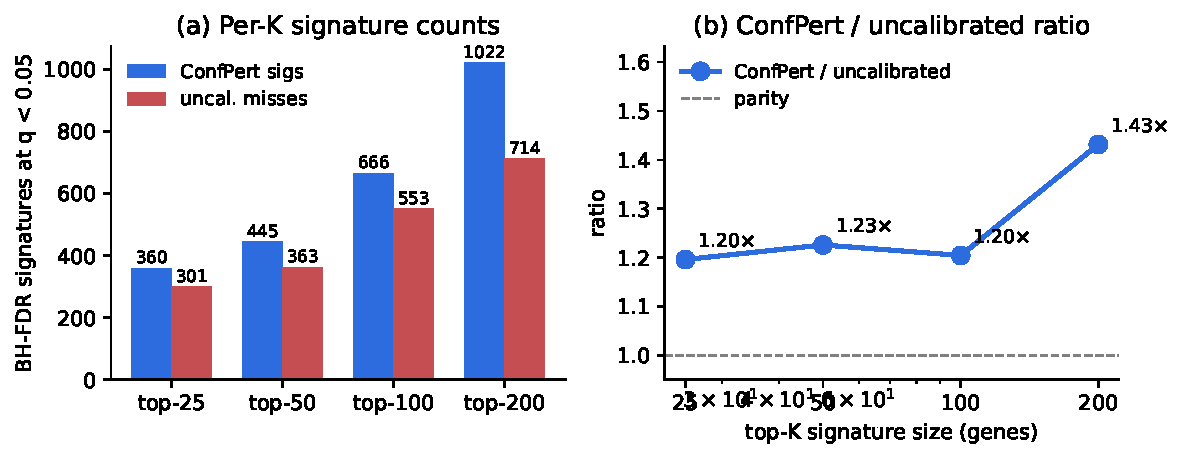
\includegraphics[width=0.95\columnwidth]{fig_k3_robustness.pdf}
\caption{K3 top-$K$ signature-size robustness. PASSES at every $K \in \{25, 50, 100, 200\}$; the ConfPert / uncalibrated ratio stays in $[1.20\times, 1.43\times]$.}
\label{fig:k3-robust}
\end{figure}

\section{Discussion}

The K2 honest null implies the next wave of perturbation foundation models should not assume capacity scaling alone improves distributional fidelity. Three implications. (i) \textbf{Calibration-aware training} (conformal-aware losses, post-hoc temperature scaling) is at least as important as capacity scaling for distributional fidelity. (ii) \textbf{Architecture choice matters more than parameter count}: sVAE+'s sparse-additive structure recovers bimodality EXACTLY at $0.800$ nominal; GEARS's marginal-Gaussian head cannot (bimodality coefficient bound $1/3 < 5/9$ by construction). (iii) \textbf{Data scale (Tahoe-100M) is the right axis} for the Virtual Cell Challenge ecosystem, not parameter scale alone. The cross-cell-line transfer split (Appendix~\ref{app:xcl}) further shows that scGen's latent-space per-perturbation delta encoding transfers across cell lines (bimodality $0.914$ exceeds the $0.80$ target), while biolord's trained variance head fully collapses under K562 $\rightarrow$ RPE1 shift --- empirical evidence for the shift-fragility documented by \citet{tibshirani2019} and motivating weighted CP.

\section{Library, Limitations, Reproducibility}

\paragraph{Library + Cell-Eval plug-in.} \texttt{confpert} is pip-installable; 4 modules + 4 dataset loaders + 33/33 unit tests. Public API: \texttt{SCORES}, \texttt{PerturbationConformal}, \texttt{CDSplitConformal}, \texttt{CauchoisSubgroupConformal}, \texttt{RCPSCalibrator}. Audit at \texttt{ArcInstitute/cell-eval}@\texttt{2db6b9c6}: 5 of 6 ConfPert discrepancies absent from the upstream registry; our \texttt{confpert.cell\_eval\_plugin} module auto-registers them.

\paragraph{Limitations.} (i) \textbf{Marginal, not conditional coverage}: ConfPert guarantees finite-sample marginal coverage; conditional coverage at every $x$ is impossible distribution-free \citep{vovk2012}. (ii) \textbf{Cross-cell-line CP is undercoverage by design}; \citet{tibshirani2019} weighted CP is exposed but enabling per-domain weights is future work. (iii) PRISM + Tahoe are cancer corpora; transfer to primary cells unsupported. (iv) Wet-lab validation excluded by pre-registration.

\paragraph{Reproducibility.} Pre-registration is git-stamped at \texttt{c7046e4b} (2026-05-03 01:30 EDT) before any Phase 1 first run. Each row of \texttt{baselines/results.json} carries a SHA-256 fingerprint. All Modal entrypoints accept \texttt{--dataset \{norman, replogle\_k562, replogle\_rpe1, adamson, tahoe\}}. Random seed $42$. 33/33 unit tests pass.

\bibliographystyle{icml2026}
\bibliography{refs}

\end{document}
